\subsection{YOLOv4}
\begin{frame}{}
    \LARGE Object Detection: \textbf{YOLOv4}
\end{frame}

\begin{frame}[allowframebreaks]{YOLOv4}
    \begin{figure}
        \centering
        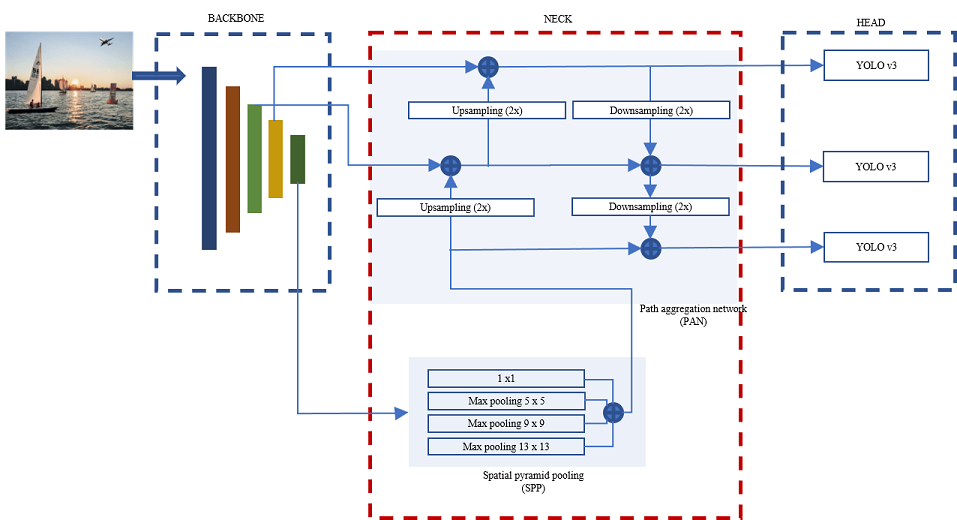
\includegraphics[width=1.0\textwidth,height=0.76\textheight,keepaspectratio]{images/object-detect/yolo-v4.png}
        \caption*{\scriptsize Source: MathWorks, ``Getting Started with YOLO v4'', MATLAB Computer Vision Toolbox documentation.}
    \end{figure}
\framebreak
    \textbf{YOLOv4 (2020):} A community-driven upgrade to YOLOv3, introducing several enhancements:
    \begin{itemize}
        \item \textbf{Backbone:} CSPDarknet53 for improved feature extraction.
        \item \textbf{Activation:} Mish activation function for better non-linearity.
        \item \textbf{Neck:} Spatial Pyramid Pooling (SPP) and PANet for multi-scale feature aggregation.
        \item \textbf{Loss:} CIoU loss for more accurate bounding box regression.
        \item \textbf{Training Tricks:} Bag-of-Freebies and Bag-of-Specials to boost performance without increasing inference cost.
    \end{itemize}
\framebreak
    \textbf{Performance:}
    \begin{itemize}
        \item 43.5\% AP (65.7\% AP@50) on COCO.
        \item $\sim$65 FPS on a Tesla V100, i.e.\ real-time.
    \end{itemize}
    \textbf{Limitation:} Relies on many training and architectural tricks, making it more complex to fully understand and implement.
\end{frame}
